% imgmlp_paper.tex -- Whole image + measurements -> MLP -> detection-based GNN (code: imgmlp/).
% Compile on Overleaf (pdfLaTeX). Results marked % RESULTS-PENDING come from logs/run_imgmlp.bat on PC1
% (results/imgmlp/*/summary.csv and probe_*.csv).
\documentclass[conference]{IEEEtran}
\usepackage[utf8]{inputenc}
\usepackage[T1]{fontenc}
\usepackage{amsmath,amssymb,amsfonts}
\usepackage{booktabs}
\usepackage{graphicx}
\usepackage{xcolor}
\usepackage{tikz}
\usetikzlibrary{arrows.meta,positioning,fit,calc}
\usepackage{url}

\newcommand{\pending}{\textcolor{gray}{--}}
\newcommand{\R}{\mathbb{R}}
\newcommand{\relu}{\operatorname{ReLU}}
\newcommand{\vect}{\operatorname{vec}}

\begin{document}

\title{Whole Images and Sensor-Agnostic Measurements for Multi-Robot Box Association:\\
an MLP Image Encoder Feeding a Detection-Based Graph Network}

\author{\IEEEauthorblockN{Alessio Martinelli}
\IEEEauthorblockA{University of L'Aquila}}

\maketitle

\begin{abstract}
A team of robots observes a static scene of identical boxes and must estimate how many boxes there are and where.
The central difficulty is association: deciding which measurements of different robots belong to the same box.
We relax the input of the learned fusion to three raw quantities per robot: its whole camera image, only resized
and converted to grey; the distance and bearing $(\rho,\theta)$ of every object it measured, from any sensor; and its
planar pose $(x,y,\psi)$. Every hand-made feature of earlier models (viewing angle of the marker, range and bearing
calibration inside the model, floor position, class) is removed from the input. A multilayer perceptron (MLP) maps
each whole image to $k$ features, and a graph neural network (GNN) with one node per measurement fuses measurements,
poses and image features into a box count and box positions. We define the input and feature spaces formally, give
two ways of bringing the image into the graph (features appended to every measurement node, or a heterogeneous graph
with one node per robot), and two geometry modes (a fixed, untrained geometric layer, or none at all). The model is
trained only in simulation, on rendered images and simulated measurements, and tested on 444 real scenes.
\textcolor{gray}{[Results: RESULTS-PENDING.]}
\end{abstract}

% ====================================================================
\section{Introduction}
% ====================================================================

Earlier models of this work fused hand-made per-detection feature vectors: a fiducial marker detector gave distance,
bearing and viewing angle, a calibration fitted on the real runs corrected them, and the floor position of every
detection was computed before the network saw it. Every one of those steps encodes a design decision about the
sensor. This paper asks what a fusion network can do when it is given only what any robot has, whatever its
sensors: an image, a list of measured objects, and its own pose.

The design follows three constraints.
\begin{enumerate}
\item \emph{No image processing before the network.} The image is only resized and converted to grey; no detector,
segmenter or hand-made descriptor is applied. The network has to discover what to extract.
\item \emph{Sensor-agnostic measurements.} A measurement is a pair $(\rho,\theta)$. Whether it comes from a fiducial
marker, an object detector or a range sensor does not change the model.
\item \emph{Scalability.} The image encoder is an MLP and not a convolutional network, and its cost per robot does not
depend on the size of the team or of the scene.
\end{enumerate}

The contributions are: (i) a formal definition of the input space and of the learned feature space;
(ii) an MLP image encoder trained end to end through a detection-based GNN; (iii) two ways of injecting the image
into the graph (graph A and graph B) and two geometry modes (fixed and strict); (iv) a protocol to choose and explain
the number of image features $k$ (sweep and linear probe), and to measure the gap between simulation and the real
scenes.

% ====================================================================
\section{Problem and input space}
% ====================================================================

\subsection{Scene}
A scene contains $N$ robots and $M$ boxes. Box $m$ has centre $b_m\in\R^2$; $M$ and $\{b_m\}$ are unknown. Each robot
$i\in\{1,\dots,N\}$ stands still and provides exactly three inputs.

\paragraph{Pose} $p_i=(x_i,y_i,\psi_i)\in\R^2\times(-\pi,\pi]$, the planar pose of its camera (OptiTrack on the real
robots).

\paragraph{Image} $I_i\in\{0,\dots,255\}^{H\times W}$, the whole grey camera frame, area-resampled from
$1280\times720$ to $W\times H$ (default $64\times36$, so $HW=2304$; also $128\times72$, $HW=9216$). Nothing else is
done to the image.

\paragraph{Measurements} a set $\mathcal{M}_i=\{(\rho_a,\theta_a)\}_{a}$ of $n_i\ge0$ measured objects, with range
$\rho_a>0$ [m] and bearing $\theta_a$ [rad], positive to the right of the optical axis, so that the world direction
of measurement $a$ is $\psi_i-\theta_a$. $n_i=0$ is allowed. A measurement can be a false report (no box), and a box
can be missed.

The full input of a scene is therefore
\begin{equation}
\mathcal{X}=\bigl\{(p_i,\,I_i,\,\mathcal{M}_i)\bigr\}_{i=1}^{N},
\end{equation}
with $n=\sum_i n_i$ measurements in total. We write $r(a)$ for the robot that produced measurement $a$.

\subsection{Output and metric}
The model returns a set of box estimates $\{\hat b_1,\dots,\hat b_{\hat M}\}$. A scene is \emph{correct} if
$\hat M=M$ and every true box has an estimate within $0.15$\,m after optimal one-to-one matching. This is the metric
of all the other methods of the thesis.

\subsection{What is not in the input}
Compared with the marker network, the following are removed: the viewing angle of the marker, the calibration of
range and bearing applied inside the model, the floor position of every detection given as a feature, and the
object class. On the real scenes the measurements are those of the fiducial marker detector after its own range and
bearing calibration. The calibration is treated as part of the sensor (what a calibrated sensor delivers), not as an
input of the model.

% ====================================================================
\section{Measurement sources}
% ====================================================================

The model never sees which source produced $(\rho,\theta)$. Three sources are used in simulation.

\paragraph{Visibility} Box $m$ is in view of robot $i$ if $0.15\le\|b_m-(x_i,y_i)\|\le3.0$\,m and
$|\theta|\le44^\circ$ (horizontal field of view $88^\circ$). It is \emph{hidden} if the segment from the camera to
$b_m$ crosses the footprint of another box, of an obstacle, or of another robot ($0.32\times0.24$\,m, centre
$0.15$\,m behind the camera).

\paragraph{Ideal} Every visible, non-hidden box is measured exactly at its centre:
$\rho=\|b_m-(x_i,y_i)\|$, $\theta=\psi_i-\operatorname{atan2}(b_m-(x_i,y_i))$, wrapped to $(-\pi,\pi]$.

\paragraph{Noisy} The ideal measurement with, per robot, a range scale error $s_i\sim\mathcal N(0,0.02^2)$ and a
bearing offset $\beta_i\sim\mathcal N(0,(1^\circ)^2)$, and per measurement
\begin{align}
\rho' &= \rho\,(1+s_i)+\varepsilon_\rho,\quad \varepsilon_\rho\sim\mathcal N\bigl(0,(0.02+0.03\rho)^2\bigr),\\
\theta' &= \theta+\beta_i+\varepsilon_\theta,\quad \varepsilon_\theta\sim\mathcal N\bigl(0,(1.5^\circ)^2\bigr).
\end{align}
A visible box is missed with probability $0.10$. Each robot adds $\operatorname{Poisson}(0.15)$ false measurements,
uniform in range $[0.15,3]$\,m and in the field of view.

\paragraph{Sensor} The detections of the fitted fiducial marker sensor model of the simulator (detection probability
against viewing angle and distance, errors along and across the line of sight, second faces, false detections),
corrected with the same calibration as the real runs.

% ====================================================================
\section{Image encoder and feature space}
% ====================================================================

\subsection{Per-image standardization}
Let $v_i=\vect(I_i)\in\R^{HW}$, with mean $\bar v_i$ and standard deviation $\sigma_i$ over its pixels. The encoder
input is
\begin{equation}
\tilde v_i=\frac{v_i-\bar v_i\mathbf 1}{\sigma_i+1}.
\end{equation}
This removes the global brightness and contrast of the frame, one of the clearest differences between rendered and
real frames. The $+1$ (one grey level) keeps a flat image finite.

\subsection{MLP}
The encoder $E:\R^{HW}\to\R^{k}$ is a three-layer MLP with no activation on the output:
\begin{equation}
z_i=E(\tilde v_i)=W_3\,\relu\bigl(W_2\,\relu(W_1\tilde v_i+c_1)+c_2\bigr)+c_3,
\end{equation}
with $W_1\in\R^{256\times HW}$, $W_2\in\R^{64\times256}$, $W_3\in\R^{k\times64}$. $E$ is shared by all robots.
Its parameter count is $256\,HW+256+16{,}448+65k$, i.e.\ $607{,}048$ for
$64\times36$ and $k=8$, and $2{,}376{,}520$ for $128\times72$. Over $99\%$ of them are in $W_1$.

\subsection{Feature space}
$z_i\in\R^k$ is a global descriptor of the whole view of robot $i$. It is unconstrained: no target is given to it,
and it is shaped only by the gradient of the association, false-report and position losses of the GNN (end-to-end
training, Sec.~\ref{sec:training}). With $k=0$ the encoder is absent and the model sees the measurements and poses
alone. This is the reference that tells what the image adds.

\subsection{Why an MLP}
A row of $W_1$ is a full-image template. The MLP is not invariant to translations in the image. Where a box appears
in the frame matters, and that position is tied to the bearing of the corresponding measurement, so this is not
a limitation for this task. Its cost is one dense product per robot, $O(HW\cdot256)$, independent of $N$, $M$ and of
the number of measurements. The whole team costs $O(N\,HW)$ for the images, and the graph costs grow with the
number of edges (Sec.~\ref{sec:scale}).

\subsection{Choosing and explaining $k$}
\label{sec:choosek}
\emph{How many:} the model is trained for $k\in\{0,2,4,8,16,32\}$ with everything else fixed, and $k$ is chosen at the
knee of the correct-scene rate on the simulated validation set. \emph{Why:} a linear probe (ridge regression,
$\lambda=1$, standardized $z$, 5-fold cross-validation grouped by scene) regresses known quantities of each frame on
$z$: boxes in the field of view, hidden boxes, mean distance of the boxes in view, mean grey level, and in simulation
ambient light, floor and wall grey, and camera pitch. The cross-validated $R^2$ says how much of each quantity the
features carry, and the ridge weights say which feature carries it.

% ====================================================================
\section{Graph network}
% ====================================================================

\begin{figure}[t]
\centering
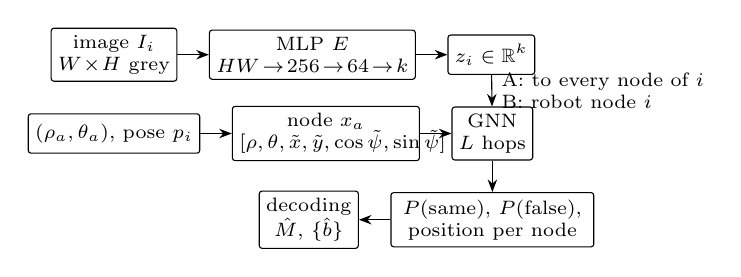
\begin{tikzpicture}[font=\scriptsize, >={Stealth[length=1.6mm]},
  box/.style={draw, rounded corners=1pt, align=center, inner sep=2.5pt, minimum height=5mm},
  det/.style={draw, circle, inner sep=1.2pt, minimum size=4.5mm},
  rob/.style={draw, rectangle, inner sep=1.2pt, minimum size=4.5mm, fill=gray!15}]
  \node[box] (img) {image $I_i$\\$W\!\times\!H$ grey};
  \node[box, right=4mm of img] (mlp) {MLP $E$\\$HW\!\to\!256\!\to\!64\!\to\!k$};
  \node[box, right=4mm of mlp] (z) {$z_i\in\R^k$};
  \node[box, below=4mm of img] (meas) {$(\rho_a,\theta_a)$, pose $p_i$};
  \node[box, right=4mm of meas, text width=22mm] (node) {node $x_a$\\$[\rho,\theta,\tilde x,\tilde y,\cos\tilde\psi,\sin\tilde\psi]$};
  \node[box, right=4mm of node] (gnn) {GNN\\$L$ hops};
  \node[box, below=4mm of gnn, text width=24mm] (out) {$P(\text{same})$, $P(\text{false})$,\\position per node};
  \node[box, left=4mm of out] (dec) {decoding\\$\hat M$, $\{\hat b\}$};
  \draw[->] (img) -- (mlp);
  \draw[->] (mlp) -- (z);
  \draw[->] (meas) -- (node);
  \draw[->] (node) -- (gnn);
  \draw[->] (z) -- node[right, align=left]{A: to every node of $i$\\B: robot node $i$} (gnn);
  \draw[->] (gnn) -- (out);
  \draw[->] (out) -- (dec);
\end{tikzpicture}
\caption{Model. The MLP turns each whole image into $k$ features. The GNN has one node per measurement; in graph B
it also has one node per robot carrying $z_i$.}
\label{fig:model}
\end{figure}

The fusion is a message-passing network~\cite{gilmer2017,battaglia2018} in which association is posed as the
classification of the edges between measurements, as in learned multi-object tracking~\cite{braso2020}.

\subsection{Normalized frame}
All positions are expressed in a frame centred at the mean robot position $c=\frac1N\sum_i(x_i,y_i)$, rotated by an
angle $\alpha$ ($\alpha=0$ at test time; drawn uniformly in $[0,2\pi)$ once per training scene) and scaled by
$R_0=1.3$\,m:
\begin{equation}
(\tilde x_i,\tilde y_i)=R_\alpha\bigl((x_i,y_i)-c\bigr)/R_0,\qquad \tilde\psi_i=\psi_i+\alpha.
\end{equation}
This is a change of coordinates, not a feature: it makes the model independent of where the arena is.

\subsection{Node features}
Each measurement $a$ is a node with
\begin{equation}
x_a=\bigl[\rho_a,\ \theta_a,\ \tilde x_{r(a)},\ \tilde y_{r(a)},\ \cos\tilde\psi_{r(a)},\ \sin\tilde\psi_{r(a)}\bigr]\in\R^6.
\end{equation}
In graph B each robot is also a node, with $u_i=[\tilde x_i,\tilde y_i,\cos\tilde\psi_i,\sin\tilde\psi_i]\in\R^4$.

\subsection{Geometry modes}
\paragraph{Fixed} A fixed layer, with no trainable parameters, computes the floor position of every measurement:
\begin{equation}
q_a=(\tilde x_{r(a)},\tilde y_{r(a)})+\frac{\rho_a}{R_0}\bigl(\cos\phi_a,\sin\phi_a\bigr),\qquad
\phi_a=\tilde\psi_{r(a)}-\theta_a,
\end{equation}
and the line-of-sight direction $\ell_a=(\cos\phi_a,\sin\phi_a)$. Two nodes are linked if $\|q_a-q_b\|\le1$\,m
(the gate). The pair $(a,b)$ carries, with $d=q_b-q_a$ (in metres, clipped at $1$\,m, in units of $0.1$\,m),
\begin{equation}
e_{ab}=\bigl[d\cdot\ell_a,\ \ell_a\times d,\ \|d\|,\ \mathbb 1[r(a)=r(b)],\ \ell_a\cdot\ell_b,\ |\ell_a\times d|\bigr]\in\R^6 .
\end{equation}
These quantities are computed from the raw inputs and are not given to the nodes. In graph B, robots closer than
$4$\,m are linked, and the edge $j\to i$ carries the offset of $j$ in the frame of $i$, $\cos$ and $\sin$ of the
heading difference, and the distance ($\R^5$).

\paragraph{Strict} No geometry is computed. Every pair of nodes of a scene is linked, with $e_{ab}=[\mathbb
1[r(a)=r(b)]]\in\R^1$; every pair of robots is linked in graph B with no edge feature. The network has to learn the
trigonometry relating $(\rho,\theta,p)$ to positions on its own.

\subsection{Graph A: image features on every node}
With $\mathcal N(a)$ the neighbours of $a$ and $L=2$ hops, hidden size $h=64$:
\begin{align}
h_a^{(0)} &= \varphi_{\text{enc}}\bigl([x_a,\,z_{r(a)}]\bigr),\\
\mu_a^{(l)} &= \operatorname{mean}_{b\in\mathcal N(a)}\ \varphi_{\text{msg}}^{(l)}\bigl([h_b^{(l-1)},\,e_{ba}]\bigr),\\
h_a^{(l)} &= h_a^{(l-1)}+\varphi_{\text{upd}}^{(l)}\bigl([h_a^{(l-1)},\,\mu_a^{(l)}]\bigr).
\end{align}
All $\varphi$ are two-layer MLPs with ReLU. A robot with $n_i=0$ has no node, so its image is not used.

\subsection{Graph B: heterogeneous, one node per robot}
Measurement nodes start from $x_a$ only, robot nodes from the pose and the image:
$h_a^{(0)}=\varphi_{\text{enc}}(x_a)$, $g_i^{(0)}=\varphi_{\text{rob}}([u_i,z_i])$. Each hop updates both kinds
simultaneously from the previous states:
\begin{align}
h_a^{(l)} &= h_a^{(l-1)}+\varphi_{\text{upd}}^{(l)}\bigl([h_a^{(l-1)},\ \mu_a^{(l)},\ \varphi_{\text{rd}}^{(l)}(g_{r(a)}^{(l-1)})]\bigr),\\
g_i^{(l)} &= g_i^{(l-1)}+\varphi_{\text{rupd}}^{(l)}\Bigl(\bigl[g_i^{(l-1)},\ \operatorname*{mean}_{a:r(a)=i}\varphi_{\text{dr}}^{(l)}(h_a^{(l-1)}),\
\operatorname*{mean}_{j\in\mathcal N_R(i)}\varphi_{\text{rr}}^{(l)}([g_j^{(l-1)},e_{ji}])\bigr]\Bigr),
\end{align}
followed by a last robot-to-measurement message $h_a\leftarrow h_a+\varphi_{\text{rd}}^{(L)}(g_{r(a)}^{(L)})$. Every
robot has a node, including one that measured nothing (on the real scenes: 45 of 1,769 robot stops). Its image then
still reaches the others. The output is still per measurement, so the model remains detection-based.

\subsection{Read-out}
For every linked pair, the same-box logit is made symmetric:
$s_{ab}=\tfrac12\bigl[\varphi_{\text{pair}}([h_a,h_b,e_{ab}])+\varphi_{\text{pair}}([h_b,h_a,e_{ba}])\bigr]$. For every node, a
false-report logit $f_a=\varphi_{\text{false}}(h_a)$ and a box position
\begin{equation}
\hat q_a=\begin{cases} q_a+0.1\,\varphi_{\text{pos}}(h_a) & \text{fixed (learned correction)}\\
\varphi_{\text{pos}}(h_a) & \text{strict.}\end{cases}
\end{equation}

\subsection{Decoding}
Nodes with $\sigma(f_a)\ge0.5$ are dropped. The rest are grouped by average-linkage agglomerative clustering on
$P_{ab}=\sigma(s_{ab})$ (unlinked pairs count as $0$), merging while the mean linkage exceeds $0.5$. Each cluster is
one box, at the mean of $\hat q_a$ over its nodes, mapped back to world coordinates. A box that no robot measured
cannot be produced. The image can therefore act on the association (merging, splitting, rejecting reports), not
on creating boxes from the image alone.

% ====================================================================
\section{Training}
\label{sec:training}
% ====================================================================

Each measurement has a label $\ell(a)\in\{1,\dots,M\}\cup\{-1\}$ (its box, or false). With $y^{\text{same}}_{ab}=\mathbb
1[\ell(a)=\ell(b)\ne-1]$ and $y^{\text{false}}_a=\mathbb 1[\ell(a)=-1]$,
\begin{equation}
\mathcal L=\operatorname{BCE}_{w_f}(f,y^{\text{false}})+\operatorname{BCE}_{w_s}(s,y^{\text{same}})
+\lambda\!\!\sum_{a:\ell(a)\ne-1}\!\!\operatorname{SmoothL1}_{\beta}\bigl(\hat q_a,\tilde b_{\ell(a)}\bigr),
\end{equation}
with positive-class weights $w=\min(10,\#\text{neg}/\#\text{pos})$ computed on the training set, $\lambda=1$,
$\beta=0.05$ (in units of $R_0$). MLP and GNN are trained together (end to end): $z$ receives no other signal.
Adam~\cite{kingma2015}, learning rate $10^{-3}$, weight decay $10^{-4}$, batches of 32 scenes, at most 40 epochs.
The epoch with the highest correct-scene rate on the validation set is kept, with early stop after 8 epochs
without improvement (strict: 60 and 12). Three seeds are trained per variant, and results are mean $\pm$ standard
deviation.

\paragraph{Data} Training: the first 20,000 scenes of the simulated training set (on average 9.5 robots and 9
boxes per scene, up to 16 of each), with one rendered frame per robot. Validation: 2,000 scenes of the same
distribution. Test: the 444 real scenes (105 layouts, 4 robots, 1,769 frames). No real scene is used for training
or for any choice.

\paragraph{Rendered images} Each simulated frame is rendered from the scene geometry by the image simulator at
$256\times144$ (the real intrinsics and lens distortion scaled, camera $0.25$\,m above the floor, pitch
$9^\circ$--$14^\circ$, the other robots, the room, and the gripper of the own robot), with exposure,
white-balance, blur, noise and JPEG effects. It is then area-resampled to $128\times72$, and to the model size when
loaded. Two looks: \emph{plain} (matched to the real room) and \emph{random} (randomized room, windows, light spots,
furniture, robot and obstacle shapes, after domain randomization~\cite{tobin2017}). The real frames are the first
reading of every robot at every stop, resampled the same way.

% ====================================================================
\section{Complexity}
\label{sec:scale}
% ====================================================================

\begin{table}[t]
\centering
\caption{Cost per scene ($N$ robots, $n$ measurements, $E$ linked pairs, $h=64$).}
\label{tab:cost}
\begin{tabular}{lll}
\toprule
Part & Cost & Grows with \\
\midrule
Image MLP & $O(N\,HW\cdot256)$ & robots \\
Graph A, fixed & $O((n+E)\,h^2)$, $E\ll n^2$ (gate) & local density \\
Graph B, fixed & $+O((N+E_R)\,h^2)$, $E_R$ within $4$\,m & local density \\
Strict & $O(n^2h^2)$ & $n^2$ \\
\bottomrule
\end{tabular}
\end{table}

With the fixed layer every node talks only to measurements within the gate, so the graph cost grows with the local
density and not with the size of the team (Table~\ref{tab:cost}). The strict mode links every pair and is quadratic
in $n$. It measures what the geometric layer is worth, and is not meant for large scenes.

% ====================================================================
\section{Experiments}
% ====================================================================

Each experiment changes one factor with respect to the reference: noisy measurements, fixed geometry, $64\times36$
images, plain look.

\begin{enumerate}
\item \emph{Number of features:} $k\in\{0,2,4,8,16,32\}$, graph A and graph B.
\item \emph{Geometry:} strict against fixed, $k\in\{0,8\}$, graph A and B.
\item \emph{Measurements:} ideal and sensor against noisy ($k=8$, graph A).
\item \emph{Resolution:} $128\times72$ against $64\times36$.
\item \emph{Sim-to-real gap:} random against plain look of the training images, with the same model evaluated on
validation (simulation) and on the real scenes.
\item \emph{Linear probe} of $z$ for every $k>0$ (Sec.~\ref{sec:choosek}).
\end{enumerate}

% ====================================================================
\section{Results}
% ====================================================================
% RESULTS-PENDING: fill from results/imgmlp/<group>/<variant>/summary.csv (rows "val" and "real":
% correct_pct +- correct_sd) and probe_<test>.csv (mean r2 over seeds).

\begin{table}[t]
\centering
\caption{Correct scenes [\%] against the number of image features $k$ (noisy measurements, fixed geometry).
Mean $\pm$ s.d.\ over 3 seeds. $k=0$: no image.}
\label{tab:sweepk}
\begin{tabular}{rcccc}
\toprule
 & \multicolumn{2}{c}{Graph A} & \multicolumn{2}{c}{Graph B} \\
\cmidrule(lr){2-3}\cmidrule(lr){4-5}
$k$ & validation & real & validation & real \\
\midrule
0  & \pending & \pending & \pending & \pending \\
2  & \pending & \pending & \pending & \pending \\
4  & \pending & \pending & \pending & \pending \\
8  & \pending & \pending & \pending & \pending \\
16 & \pending & \pending & \pending & \pending \\
32 & \pending & \pending & \pending & \pending \\
\bottomrule
\end{tabular}
\end{table}

\begin{table}[t]
\centering
\caption{Ablations: correct scenes [\%], one factor changed from the reference
(noisy, fixed, graph A, $k=8$, $64\times36$, plain look).}
\label{tab:ablation}
\begin{tabular}{lcc}
\toprule
Variant & validation & real \\
\midrule
Reference & \pending & \pending \\
Strict, graph A, $k=0$ & \pending & \pending \\
Strict, graph A, $k=8$ & \pending & \pending \\
Strict, graph B, $k=0$ & \pending & \pending \\
Strict, graph B, $k=8$ & \pending & \pending \\
Ideal measurements & \pending & \pending \\
Sensor-model measurements & \pending & \pending \\
Images $128\times72$ & \pending & \pending \\
Random look (training) & \pending & \pending \\
\bottomrule
\end{tabular}
\end{table}

\begin{table}[t]
\centering
\caption{Linear probe of the image features ($k=8$): cross-validated $R^2$, mean over seeds.}
\label{tab:probe}
\begin{tabular}{lcccc}
\toprule
 & \multicolumn{2}{c}{Graph A} & \multicolumn{2}{c}{Graph B} \\
\cmidrule(lr){2-3}\cmidrule(lr){4-5}
Quantity & sim & real & sim & real \\
\midrule
Boxes in view & \pending & \pending & \pending & \pending \\
Hidden boxes & \pending & \pending & \pending & \pending \\
Mean distance & \pending & \pending & \pending & \pending \\
Mean grey level & \pending & \pending & \pending & \pending \\
Ambient light & \pending & -- & \pending & -- \\
Camera pitch & \pending & -- & \pending & -- \\
\bottomrule
\end{tabular}
\end{table}

\paragraph{Number of features} \textcolor{gray}{[RESULTS-PENDING: knee of Table~\ref{tab:sweepk}; gain of the best
$k$ over $k=0$.]}

\paragraph{Graph A against graph B} \textcolor{gray}{[RESULTS-PENDING.]}

\paragraph{Geometric layer} \textcolor{gray}{[RESULTS-PENDING: fixed against strict.]}

\paragraph{What the features encode} \textcolor{gray}{[RESULTS-PENDING: Table~\ref{tab:probe}.]}

\paragraph{Gap between simulation and the real scenes} \textcolor{gray}{[RESULTS-PENDING: validation against real
for the plain and random looks.]}

% ====================================================================
\section{Limitations}
% ====================================================================

The model outputs boxes only where at least one measurement exists, so the image cannot recover a box that no
sensor reported. The MLP sees raw pixels, so any difference in appearance between rendered and real frames enters
the features directly. Per-image standardization removes only global brightness and contrast. The real scenes have
4 robots, fewer than the training scenes (up to 16). Colour is not used yet: the encoder takes grey images, and
colour is the next step for the real scenes.

% ====================================================================
\section{Conclusion}
% ====================================================================

\textcolor{gray}{[RESULTS-PENDING.]}

\begin{thebibliography}{9}
\bibitem{gilmer2017} J. Gilmer, S. S. Schoenholz, P. F. Riley, O. Vinyals, and G. E. Dahl, ``Neural message passing
for quantum chemistry,'' in \emph{Proc. 34th Int. Conf. Mach. Learn. (ICML)}, 2017, pp. 1263--1272.
\bibitem{battaglia2018} P. W. Battaglia \emph{et al.}, ``Relational inductive biases, deep learning, and graph
networks,'' 2018, arXiv:1806.01261.
\bibitem{braso2020} G. Brasó and L. Leal-Taixé, ``Learning a neural solver for multiple object tracking,'' in
\emph{Proc. IEEE/CVF Conf. Comput. Vis. Pattern Recognit. (CVPR)}, 2020, pp. 6247--6257.
\bibitem{tobin2017} J. Tobin, R. Fong, A. Ray, J. Schneider, W. Zaremba, and P. Abbeel, ``Domain randomization for
transferring deep neural networks from simulation to the real world,'' in \emph{Proc. IEEE/RSJ Int. Conf. Intell.
Robots Syst. (IROS)}, 2017, pp. 23--30.
\bibitem{kingma2015} D. P. Kingma and J. Ba, ``Adam: A method for stochastic optimization,'' in \emph{Proc. Int.
Conf. Learn. Represent. (ICLR)}, 2015.
\end{thebibliography}

\end{document}
